\documentclass[12pt]{article}
\usepackage{preamble}

\pagestyle{fancy}
\fancyhead[LO,LE]{Математический анализ}
\fancyhead[CO,CE]{21.02.2024}
\fancyhead[RO,RE]{Лекции Далевской О. П.}


\begin{document}

    \section{2. Несобственные интегралы}

    \section{2.1 Определения}

    \textbf{1* Интегралы на неограниченном промежутке}

    Геометрический смысл: пусть $f(x) : [a; +\infty] \to \Real$, $\displaystyle f(x) \in C_{[a; +\infty]}$

    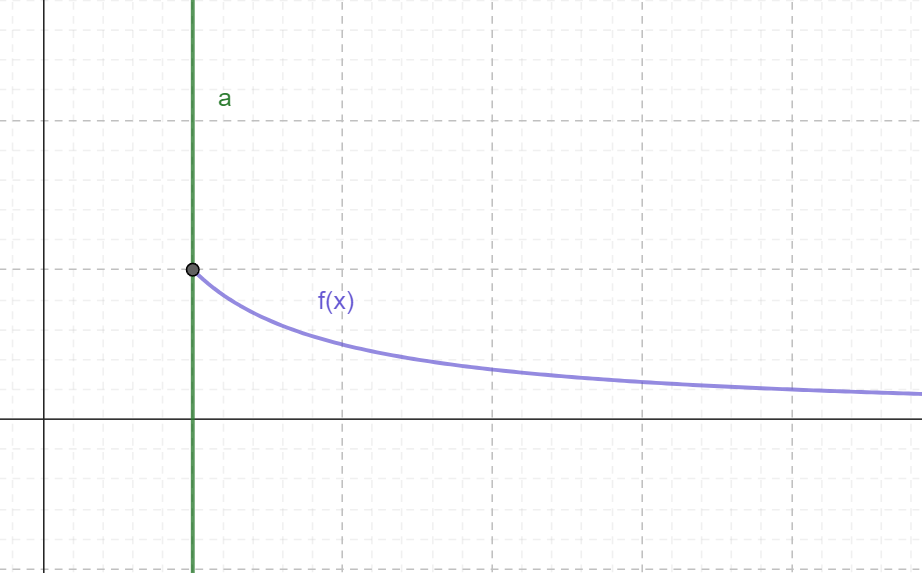
\includegraphics[height=90mm]{images/calculus_2024_02_21_1}

    Тогда определенный интеграл имеет смысл - это площадь под графиком функции:

    \[\int^{b}_{a} f(x) dx = S\]

    Имеет ли смысл площадь неограниченной фигуры под графиком функции?

    Предел функции $\displaystyle \Phi (b) = \int^{b}_{a} f(x) dx$ при $b \to +\infty$ может быть конечным или бесконечным

    \DefN{1} Определим несобственный интеграл первого рода (на неограниченном промежутке) ($f(x)$ любого знака):

    \[\int^{+\infty}_{a} f(x) dx = \lim_{b \to +\infty} \int^{b}_{a} f(x) dx\]

    \Nota Если этот предел существует и конечен, то говорят, что интеграл сходится. В противном случае расходится

    \DefN{2} Функция определена на полуинтервале $[-\infty; b]$ и непрерывна. Тогда определен:

    \[\int^{b}_{-\infty} f(x) dx = \lim_{a \to -\infty} \int^{b}_{a} f(x) dx\]

    \DefN{3} $\displaystyle \int^{+\infty}_{-\infty} f(x) dx = \int^{c}_{-\infty} f(x) dx + \int^{+\infty}_{c} f(x) dx$

    \Nota Этот интеграл сходится, если сходятся оба интеграла справа, и расходится, если расходится хотя бы один из них
    (в том числе если возникает неопределенность $\infty - \infty$)

    \Ex $\displaystyle f(x) = \frac{1}{x}$

    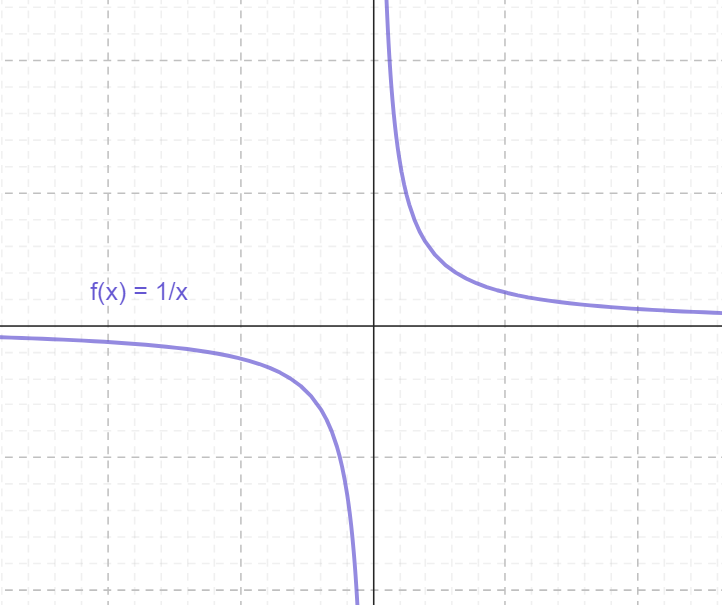
\includegraphics[height=90mm]{images/calculus_2024_02_21_2}

    Сделаем ее непрерывной

    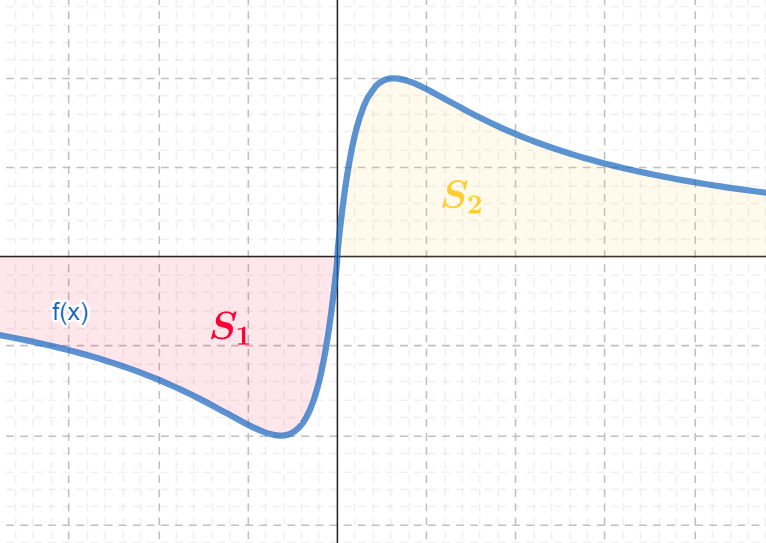
\includegraphics[height=90mm]{images/calculus_2024_02_21_3}

    $\displaystyle S_1 = S_2$, но $\displaystyle I_1 = -I_2$. Суммарный интеграл $\displaystyle \int^{+\infty}_{-\infty} f(x) dx$ должен быть равен нулю.

    Но по определению $\displaystyle \int^{+\infty}_{-\infty} f(x) dx$ расходится

    Чтобы учесть обнуление интеграла в ситуации взаимного погашения площадей $\displaystyle S_1$ и $\displaystyle S_2$
    (а это происходит тогда, когда левый и правый концы промежутка синхронно стремятся к $+\infty$)
    используют понятие интеграла в смысле главного значения ($v.p.$ - от французского \textit{valeur principale}):

    $\displaystyle v.p. \int^{+\infty}_{-\infty} f(x) dx = \lim_{\delta \to -\infty} \int^{\delta}_{-\delta} f(x) dx$

    Разложение по формуле Ньютона-Лейбница

    \ExN{1} \[\int^{+\infty}_{-\infty} \frac{dx}{1 + x^2} = arctg x \Big|^{+\infty}_{-\infty} = arctg x \Big|^{c = 0}_{-\infty} + arctg x \Big|^{+\infty}_{c = 0} =
    \lim_{x \to +\infty} arctgx - arctg(0) + arctg(0) - \lim_{x \to -\infty} arctgx = \frac{\pi}{2} + \frac{\pi}{2} = \pi\]

    \ExN{2} \[\int^{+\infty}_{1} \frac{dx}{xlnx} = \int^{+\infty}_{1} \frac{dlnx}{lnx} = \int^{+\infty}_{0} \frac{dt}{t}
     = lnt \Big|^{+\infty}_{0} = ln ln x \Big|^{+\infty}_{1} = \lim_{x \to +\infty} ln ln x - \lim_{x \to 1} ln ln x = \infty - \infty\] - расходится

    Заметим нарушение непрерывности функции $\displaystyle \frac{1}{xlnx}$ в $x = 1$, что привело к $ln lnx \to -\infty$ при $x \to 1$

    Это не интеграл первого рода, а комбинация интегралов первого и второго рода

    \textbf{2* Интеграл от неограниченной на отрезке функции}

    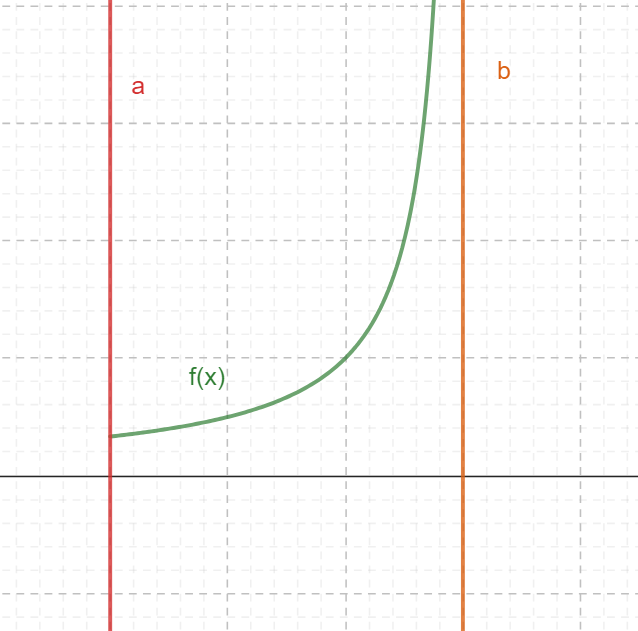
\includegraphics[height=90mm]{images/calculus_2024_02_21_4}

    $f(x) : [a; b) \to \Real$, где $b$ - точка разрыва второго рода, а именно бесконечного

    \DefN{1} Интеграл второго рода (несобственный)

    \[\int^{b}_{a} f(x) dx = \lim_{\beta \to b} \int^{\beta}_{a} f(x) dx\]

    Этот интеграл сходится, если предел существует и конечен

    \DefN{2} Аналогично ($a$ - точка бесконечного разрыва):

    \[\int^{b}_{a} f(x) dx = \lim_{\alpha \to a} \int^{b}_{\alpha} f(x) dx\]

    \DefN{3} $c \in [a;b]$ - точка бесконечного разрыва:

    \[\int^{b}_{a} f(x) dx = \int^{c}_{a} f(x) dx + \int^{b}_{c} f(x) dx\]

    Сходится, если оба интеграла сходятся

    \ExN{1}

    \[\int^{1}_{-1} \frac{dx}{x} = \int^{0}_{-1} \frac{dx}{x} + \int^{1}_{0} \frac{dx}{x} =
    ln |x| \Big|^{0}_{-1} + ln |x| \Big|^{1}_{0}\] - интеграл расходится

    Не заметили $\displaystyle \int^{1}_{-1} \frac{dx}{x} = ln |x| \Big|^{1}_{-1} = 0$ ???

    \ExN{2}

    \[\int^{1}_{-1} \frac{dx}{x^2} = -\frac{dx}{x} \Big|^{1}_{-1} = -2\] - неверно

    \[\int^{1}_{-1} \frac{dx}{x^2} = \int^{0}_{-1} \frac{dx}{x^2} + \int^{1}_{0} \frac{dx}{x^2} =
    -\frac{dx}{x} \Big|^{0}_{-1} + -\frac{dx}{x} \Big|^{1}_{0}\] - расходится

    \Nota Если нет разбиения $[a; b]$ по аддитивности, то неопределенности раскрываются

    \Ex $\displaystyle \int^{2}_{1} \frac{dx}{x^2 - 1} = \frac{1}{2} \int^{2}_{1} (\frac{1}{x - 1} - \frac{1}{x + 1})dx =
    \frac{1}{2} (ln|x - 1| - ln|x + 1|) \Big|^{2}_{1} = \\
    = \frac{1}{2} (ln|1 - 1| - ln|x + 1|) \Big|^{2}_{1} = \infty \text{,  т. к. разбивается отрезок}\\
    = \frac{1}{2} (ln|\frac{x - 1}{x + 1}) \Big|^{2}_{1} = \frac{1}{2} (ln\frac{1}{3} - ln(0)) = \infty \text{  - теперь точно } \infty
    $

    \section{2.2 Свойства}

    1) Линейность: $\displaystyle \int^{+\infty}_{a} (\lambda f(x) + \mu g(x)) dx = \lambda \int^{+\infty}_{a} f(x) dx + \mu \int^{+\infty}_{a} g(x) dx$
    - если интегралы сходятся (иначе исследуем по определению через предел)

    2) Аддитивность: $\displaystyle I = \int^{+\infty}_{a} f(x) dx = \int^{c}_{a} f(x) dx + \int^{+\infty}_{c} f(x) dx$
    - отсечение любого конечного интеграла $\displaystyle \int^{c}_{a} f(x) dx$ не влияет на сходимость

    3) Знаки интегралов:

    $\displaystyle \int^{+\infty}_{a} f(x) dx \geq \int^{+\infty}_{a} g(x) dx $ при $f(x) \leq g(x)$ и интегралы сходятся

    В частности $\displaystyle \int^{+\infty}_{a} f(x) dx \geq 0$ при $f(x) \leq 0$ на $[a; +\infty]$

    \Nota Исследование интегралов двух функций используется для определения их сходимости


    \section{2.3 Сходимость несобственных интегралов}

    Задача: Часто нужно исследовать интеграл на сходимость без или до его вычисления (обычно приближенного для неберущихся интегралов)

    Требуются признаки сходимости интегралов, часто использующие сравнение с эталонными интегралами (вычисляемые по формуле Ньютона-Лейбница)

    \textbf{2* Признак сравнения в неравенствах} (далее только для интегралов $\displaystyle \int^{+\infty}_{a} f(x) dx$, для остальных аналогично)

    $\displaystyle f(x), g(x) : [a;+\infty) \to \Real^+$, непрерывны на $[a;+\infty)$ и $\forall x \in [a;+\infty) f(x) \leq g(x)$


    Тогда, если $\displaystyle \int^{+\infty}_{a} g(x) dx = I \in \Real$, то $\displaystyle J = \int^{+\infty}_{a} f(x) dx$ сходится,
    причем $\displaystyle0 \leq \int^{+\infty}_{a} f(x) dx \leq \int^{+\infty}_{a} g(x) dx$

    Прежде чем использовать свойство ОИ и предельный переход в неравенства,
    нужно доказать, что интеграл $\displaystyle J = \lim_{b \to +\infty} \int^{b}_{a} f(x) dx$ сходится

    Т. к. $f(x) \geq 0$, то $\displaystyle \int^{b}_{a}f(x)dx$ при $b \to \infty$ монотонно возрастающая функция

    При этом:

    \[0 \leq \int^{b}_{a}f(x)dx \leq \int^{b}_{a}g(x)dx \leq \lim_{b \to +\infty} \int^{b}_{a}g(x)dx = I \in \Real\]

    То $\displaystyle J(b) = \int^b_a f(x)dx$ ограничена и по признаку Вейерштрасса сходится

    Можно использовать предельный переход

    \[0 \leq \int^{b}_{a}f(x)dx \leq \int^{b}_{a}g(x)dx \quad \Big| \lim_{b \to +\infty}\]

    \[0 \leq J \leq I\]

    \Nota Можно аналогично сравнить функции отрицательного знака

    Если сходится $\displaystyle \int^{+\infty}_{a} g(x) dx$ при $g(x) \leq f(x) \leq 0$, то сходится $\displaystyle \int^{+\infty}_{a} f(x) dx$

    Интегралы от функций разных знаков этим методов не сравниваются

    $f(x) \leq g(x) \forall x \in [a;+\infty)$, но функции разных знаков, и нижняя площадь, т. е. $\displaystyle \int^{b}_{a} |f(x)| dx$, больше верхней

    \textbf{1* $\displaystyle f(x), g(x) \in C_{[a;+\infty)}$, $0 \leq f(x) \leq g(x) \forall x \in [a;+\infty)$}

    $\displaystyle J = \int^{+\infty}_{a} f(x) dx \text{  расходится. Тогда  } I = \int^{+\infty}_{a} g(x) dx \text{  расходится}$

    $\Box$ \Lab (от противного)

    \Nota Отметим, что если $f(x)$ не является убывающей к нулю, т. е. б. м. на $+\infty$, то $\displaystyle \int^{+\infty}_{a} f(x) dx$ разойдется

    Таким образом, если сравнить б. м. $\displaystyle \frac{f(x)}{g(x)}$, то можно исследовать их интегралы на сходимость

    \textbf{2* Предельный признак сравнения}

    $\displaystyle f(x), g(x) \in C_{[a;+\infty)}$, $f(x), g(x) > 0$

    $\displaystyle \exists \lim_{x\to+\infty} \frac{f(x)}{g(x)} = k \in \Real \Setminus \Set{0}$.
    Тогда $\displaystyle I = \int^{+\infty}_{a} g(x)dx$ и $\displaystyle J = \int^{+\infty}_{a} f(x)dx$ одновременно сходятся или расходятся

    $\displaystyle \Box \lim_{x\to+\infty} \frac{f(x)}{g(x)} = k \Longleftrightarrow \forall \varepsilon > 0 \exists \delta > 0 | \forall x > \delta |\frac{f(x)}{g(x)} - k| < \varepsilon $

    $\displaystyle -\varepsilon + k < \frac{f(x)}{g(x)} < \varepsilon + k \quad \Big| * g(x) > 0$

    $\displaystyle (k - \varepsilon)g(x) < f(x) < (\varepsilon + k)g(x)$

    Т. к. $k > 0$ ($\displaystyle \frac{f(x)}{g(x)} > 0$) и $\varepsilon$ - сколь угодно мало, то $k \pm \varepsilon$ - положительное и не близкое к нулю число

    ОИ: $\displaystyle \int^{b}_{a} (k - \varepsilon)g(x) dx < \int^{b}_{a} f(x) dx < \int^{b}_{a} (k + \varepsilon)g(x) dx$

    $\displaystyle \lim_{b \to +\infty}$: $\displaystyle (k - \varepsilon) \int^{+\infty}_{a} g(x) dx < \int^{+\infty}_{a} f(x) dx < (k + \varepsilon) \int^{+\infty}_{a} g(x) dx$

    Если $I = \infty$ (но $k - \varepsilon \neq 0$), то по первому признаку (линейность) $J$ расходится
    Если $I \in \Real$ ($k + \varepsilon \neq \infty$), то по первому признаку (линейность) $J$ сходится

    \textbf{3* Абсолютная сходимость}

    $\displaystyle \int^{+\infty}_{a} |f(x)| dx = I \in \Real \Longrightarrow \int^{+\infty}_{a} f(x) dx = J \in \Real$

    \Nota Обратное неверно

    $\Box$ ОИ и модуль:

    \[\int^{b}_{a} f(x) dx \leq |\int^{b}_{a} f(x) dx| \leq \int^{b}_{a} |f(x)| dx\]

    Очевидно, что $\displaystyle 0 \leq |\int^{b}_{a} f(x) dx| \leq \int^{b}_{a} |f(x)| dx \leq \lim_{b \to \infty} \int^{b}_{a} |f(x)| dx = I$

    \[-I \leq \int^{b}_{a} f(x) dx \leq I\]

    \[0 \leq \lim_{b \to \infty}|\int^{b}_{a} f(x) dx| = |\lim_{b \to \infty} \int^{b}_{a} f(x) dx| \leq \int^{b}_{a} |f(x)| dx = I\]

    \Nota Если $\displaystyle I = \int^{+\infty}_{a} f(x) dx$ сходится, но $\displaystyle |\int^{+\infty}_{a} f(x) dx|$ расходится, то $I$ называют условно сходящимся

    \Ex $\displaystyle I = \int^{+\infty}_{a} \frac{sinx}{8x^2 + 3} dx$

    $\displaystyle \int^{+\infty}_{a} |\frac{sinx}{8x^2 + 3}| dx = \int^{+\infty}_{a} \frac{|sinx|}{8x^2 + 3} dx \text{синус ограничен} \leq \int^{+\infty}_{a} \frac{dx}{8x^2 + 3} dx = \frac{1}{k} arctg\frac{x}{k} \Big|^{+\infty}_{1} \in \Real$

    В качестве эталонных интегралов удобно использовать:

    I рода: $\displaystyle \int^{+\infty}_{a} \frac{dx}{x^n}$

    II рода: $\displaystyle \int^{b}_{a} \frac{dx}{(b - x)^n}$

    \Lab Исследовать на сходимость в зависимости от $n \in \Integer (\Rational)$

    \clearpage

    \section{3. Интегралы зависящие от параметра}

    Задача. Ex ($\alpha \neq 0$). $\displaystyle \int^{1}_{0} cos\alpha x dx = \frac{1}{\alpha} \int^{1}_{0} cos\alpha x d\alpha x = \frac{1}{\alpha} sin \alpha x \Big|^{1}_{0} = \frac{sin\alpha}{\alpha} = \phi(\alpha)$

    $\displaystyle J(\alpha) = \int^b_a f(x, \alpha)dx$ - интеграл, зависящий от параметра

    $f(x, \alpha)$ непрерывна в $a \leq x \leq b$, $c \leq \alpha \leq d$ и существует непрерывная производная $\displaystyle f^\prime_\alpha$

    Тогда на $[c;d]$ определена $\displaystyle J^\prime_\alpha(\alpha) = \left(\int^b_a f(x, \alpha)dx\right)^\prime_\alpha = \int^b_a f^\prime_\alpha dx$

    Если последний интеграл берется лучше, чем исходный, то теорема полезна

    $\displaystyle \Box J^\prime_\alpha(\alpha) = \lim_{\Delta \alpha \to 0} \frac{J(\alpha + \Delta \alpha) - J(\alpha)}{\Delta \alpha} =
    \lim_{\Delta \alpha \to 0} \frac{1}{\Delta \alpha} (\int^b_a f(x, \alpha + \Delta \alpha)dx - \int^b_a f(x, \alpha)dx) =
    = \lim_{\Delta \alpha \to 0} \frac{1}{\Delta \alpha} (\int^b_a (f(x, \alpha + \Delta \alpha) - f(x, \alpha))dx)$

    По теореме Лагранжа о среднем $\exists \xi \in [\alpha; \alpha + \Delta \alpha]$

    $\displaystyle = \lim_{\Delta \alpha \to 0} \int^b_a f(x, \xi)dx$

    Т. к. $\displaystyle f^\prime_\alpha$ непрерывна, то $\displaystyle f^\prime_\alpha (x, \xi) = \lim_{\xi \to \alpha} f^\prime_\alpha (x, \xi) + \varepsilon = f^\prime_\alpha (x, \alpha) + \varepsilon$

    Таким образом $\displaystyle J^\prime_\alpha(\alpha) = \lim_{\Delta \alpha \to 0} \int^{b}_{a} f^\prime_{\alpha}(x, \alpha) dx + \lim_{\Delta \alpha \to 0} \int^{b}_{a} \varepsilon dx =
    \lim_{\Delta \alpha \to 0} \int^{b}_{a} f^\prime_{\alpha}(x, \xi) dx$


\end{document}
